\documentclass[11pt]{article}
\usepackage{amsfonts,amsmath,amssymb,amsthm} % Math packages
\usepackage{graphicx} % For including images
\usepackage{titlesec} % For customizing section titles
\usepackage{titling} % For customizing the title
\usepackage{geometry} % For adjusting page margins
\usepackage{datetime} % For formatting the date
\usepackage{hyperref} % For adding hyperlinks


% Customize the title format
\pretitle{\begin{center}\Large\bfseries}
\posttitle{\par\end{center}}
\preauthor{\begin{center}\large}
\postauthor{\end{center}}
\predate{\begin{center}\large}
\postdate{\par\end{center}}

% Customize the section title format
\titleformat{\section}{\large\bfseries}{\thesection.}{0.5em}{}

% Adjust the page margins
\geometry{margin=1in}

\begin{document}

% Create the title page
\begin{titlepage}
    \centering
    \vspace*{0.5cm}
    \par\normalfont\fontsize{35}{35}\sffamily\selectfont
    Assignment 03 - MATH 525\par 
    \vspace*{1cm}
    {\huge\bfseries Huzaifa Unjhawala \\  Gabe Selzer \par} 
    \vspace*{1cm}
    {\Large\itshape Date: \today\par} 
    \vfill
\end{titlepage}

\section*{Problem 1}

Consider any point $y\in S$. We will show that $f(x^*)\leq f(y)$.

We know that $x^*$ is a local minimum, i.e. that $\exists\epsilon>0$ such that $\forall x\in S, ||x-x^*||\leq \epsilon$ we have $f(x^*)\leq f(x)$. If $||y-x^*||\leq \epsilon$, then by the definition of a local minimum we know $f(x^*)\leq f(y)$. Thus the only remaining case to consider is when $||y-x^*||>\epsilon$

Consider $a=\frac{\epsilon}{||y-x^*||}\in\mathbb{R}$. Since $\epsilon> 0$ and $||y-x^*||>\epsilon$, it must hold that $0<a<1$, or equivalently that $a\in[0, 1]$.

Consider the point $z=ay + (1-a)x^*$, a convex combination of $y$ and $x^*$. Since $S$ is a convex set, $z\in S$. We have

\begin{equation}
\begin{split}
||z-x^*|| &= ||\bigl(ay + (1-a)x^*\bigr) - x^*|| \\
&= ||\bigl(ay + x^*-ax^*\bigr) - x^*|| \\
&= ||ay -ax^*|| \\
&= a||y -x^*|| \\
&= \frac{\epsilon}{||y-x^*||}||y -x^*|| \\
&= \epsilon\\
\end{split}
\end{equation}

Since $||z-x^*|| = \epsilon$ we have $f(x^*)\leq f(z)$. Since $f$ is a convex function, we know that

\begin{equation}
\begin{split}
f(x^*)\leq f(z) = f(ay + (1-a)x^*) &\leq af(y) + (1-a) f(x^*)\\
f(x^*) &\leq af(y) + (1-a) f(x^*) \\
af(x^*) &\leq af(y) \\
f(x^*) &\leq f(y) \\
\end{split}
\end{equation}

Note that the last step only holds as $a$ must be positive. Thus $\forall y\in S$, we know $f(x^*)\leq f(y)$. By definition, $x^*$ is a global maximum. Q.E.D. 

\section*{Problem 2}

We note that Theorem 2.6 from the lecture notes states that a polyhedron contains an extreme point if and only if it contains a line.

Standard form problems cannot possibly contain a line, as they are confined as a subset of the positive orthant $\{x|x\geq 0\}$. This is not a requirement of general form problems, and as such they can contain a line. For example, the polyhedron $P=\{x\in\mathbb{R}^2|x_1\geq 4\}$ comprises a half-space, containing many lines (such as $x_1=5$).

Just because we can turn a general form polyhedron into a standard form polyhedron with the same optimal cost, this does not mean that the polyhedron is equivalent. By transforming a polyhedron into standard form, we add dimensions such that we can maintain the constraints of the original problem through a polyhedron in the positive orthant. The fact that the general form polyhedron and the standard form polyhedron (may) lie in different dimensionalities is enough to reason that they may not be equivalent, despite leading to an equivalent LP problem. For this reason, we cannot conclude that every nonempty polyhedron contains an extreme point. \\
Additionally, we can also reason with the help of an example where we first show a LP problem defined in standard form which contains a line and thus no vertex. We then define a equivalent LP problem in standard form which does not contain a line and thus has a vertex. \\
Consider a polyhedron given by
\[ P_2 = \{ \textbf{x} \in \mathbb{R}^5 | x_1-x_2+x_3-x_4 - x_5 = 0, \textbf{x} \ge 0\}\]
This polyhedron thus has a vertex at \(\textbf{0} \in \mathbb{R}^5\). Now this same LP problem can be expressed equivalently in general form with the feasible set described by the polyhedron 
\[P_2 = \{\textbf{x} \in \mathbb{R}^2 | x_1 + x_2 \ge 0\}\]
This polyhedron contains a line \(x_1 + x_2 = 0\). Thus, we can see that all though the two LP problems are equivalent, the feasible set is geometrically very different.


\section*{Problem 4}

We have $P=\{x\in\mathbb{R}^n: a_i'x=b_i, i=1...m\}$, where P is bounded and $m\geq n$. We also have $Q=\{x\in P: a'x=b\}$ for some $a\in\mathbb{R}^n, b\in\mathbb{R}$. We show that every extreme point of $Q$ is either an extreme point of $P$ or a convex combination of two adjacent extreme points of $P$.\\

Suppose that $Q$ has an extreme point $x^*$. Since $x^*$ is an extreme point, Theorem 2.3 from the lecture notes tells us that there are $n$ linearly independent constraints active at $x^*$. We know from the definition of $Q$ that $a'x=b$ is active at $x^*$, thus the remaining constraints active at $x^*$ must come from the constraints of $P$. Let $I(x^*)=\{i\in\{1...m\}:a_i'x=b_i\}$ define these remaining constraints from $P$. Note that $a$ may or may not be linearly independent with this set, so we consider each case:\\

\underline{$a$ is linearly dependent with $\{a_i:i\in I(x^*)\}$}\\

If $a$ is linearly dependent with this set, then the $n$ linearly independent constraints must all lie in $\{a_i:i\in I(x^*)\}$, and $x^*$ is also an extreme point of $P$.\\

\underline{$a$ is linearly independent with $\{a_i:i\in I(x^*)\}$}\\

If $a$ is linearly independent with this set, then of the $n$ linearly independent constraints active at $x^*$ in $Q$, $(n-1)$ of them must come from  $\{a_i:i\in I(x^*)\}$. These $(n-1)$ linearly independent constraints \textbf{do not span} $\mathbb{R}^n$, and there must exist some nonzero $d\in\mathbb{R}^n$ such that $\forall i\in I(x^*)\quad a_i'd=0$.\\

Let $y=x^*+\lambda d$. $\forall \lambda\in\mathbb{R}, i\in I(x^*)$, we have $a_i'y=a_i'x^*+\lambda a_i'd$. Since $a_i'd=0$, we have $a_i'y = a_i'x^*=b_i$. Thus $I(y)\supseteq I(x^*)$ for any $y$. \\

$Q$ is bounded, meaning that if we travel in the direction of any nonzero vector from $x^*$ we must eventually reach a constraint. This is easily shown from the definition of a bounded polyhedron, keeping in mind that we are adding a nonzero vector to a point in $Q$.\\

Suppose, going in the direction of $d$, we find some $\lambda^+>0, j\notin I(x^*)$ at which $a_j'(x^*+\lambda^+d)=b_j$. $a_j$ cannot be expressed as a linear combination of $\{a_i: i\in I(x^*)\}$. This is because $a_i'd=0$ for all $a_i$, and

$$
a_j'(x^*)>b_j \text{ and } a_j'(x^* + \lambda^+ d) = b_j \Rightarrow a_j'd \neq 0\\
$$

Thus $\{a_i: i\in I(x^*)\cup\{j\}\}$ contains $n$ linearly independent vectors, and we have $y^+=x^*+\lambda^+ d$ is an extreme point.\\

Similarly, we can go in the direction $-d$, until, for some $\lambda^-> 0, k\notin I(x^*)$ at which $a_k'(x^*-\lambda^-d)=b_k$, and we find that $a_k$ is also linearly independent from $\{a_i\}$, making  $y^-=x^*-\lambda^- d$ is an extreme point. We note that $y^+$ and $y^-$ share $(n-1)$ active constraints, and that $y^+\neq y^-$, as
$$
y^+-y^-=x^*+\lambda^+ d - (x^*-\lambda^- d) = d(\lambda^++\lambda^-)>0
$$
Thus $y^+$ and $y^-$ are distinct adjacent basic feasible solutions. Furthermore, since $x^*$ lies on the line segment between $y^+$ and $y^-$, it can be expressed as a linear combination of the two, with

\begin{equation}
\begin{split}
x^* &= by^+ + (1-b)y^-\\
x^* &= bx^* + b\lambda^+d + x^* - \lambda^-d - bx^* + b\lambda^-d\\
0 &= b\lambda^+d - \lambda^-d + b\lambda^-d\\
\lambda^-d &= b(\lambda^+d+\lambda^-d)\\
b&=\frac{\lambda^-}{\lambda^+ + \lambda^-}
\end{split}
\end{equation}

Since $\lambda^->0, \lambda^+>0$, we know that $0<b<1$, and $x^*$ is actually a convex combination of two adjacent extreme points of $P$, $y^+$ and $y^-$. Q.E.D.

\section*{Problem 5}

We consider this problem geometrically, by looking at a visual of $P$:

\begin{figure}[h]
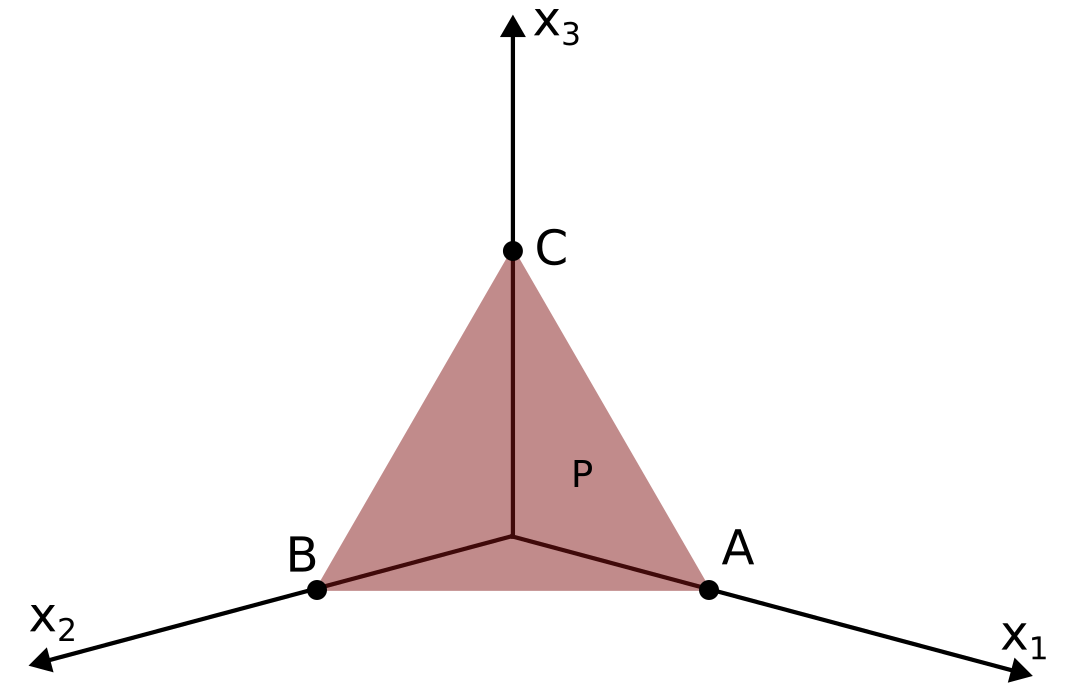
\includegraphics[width=0.5\textwidth]{5_geometry}
\centering
\caption{The geometry of $P$, along with vertices $A, B, C$}
\end{figure}

We can see three vertices of $P$, most notably, $C=\begin{bmatrix}0\\0\\1\end{bmatrix}$. From $C$, we can see that feasible directions from $C$, geometrically speaking, include going towards $B$, going towards $A$, or going in a direction in between $A$ and $B$, as shown in Figure 2.

\begin{figure}[h]
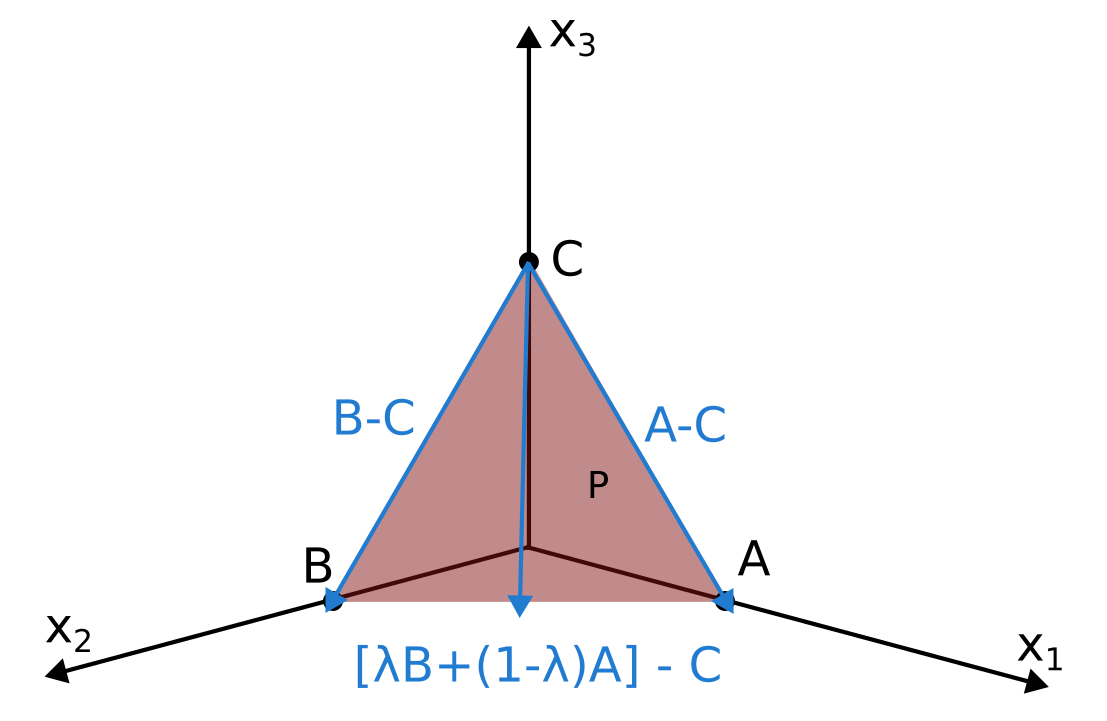
\includegraphics[width=0.5\textwidth]{5_feasible_directions}
\centering
\caption{Feasible directions from $A$}
\end{figure}

 Arithmetically speaking, any of these directions $d$ can be represented as a convex combination of $(A-C)$ and $(B-C)$: 

\begin{equation}
d=\lambda(A-C) + (1-\lambda) (B-C); \lambda\in[0, 1]
\end{equation}

Arithmetically speaking, we can only prove that $d$ is a feasible solution at $C$ if $y=C+\theta d\in P$ for some positive $\theta$:

\begin{equation}
\begin{split}
y &= C + \theta d\\
y &= C + \theta\bigl[\lambda (A-C) + (1-\lambda) (B-C)\bigr]\\
y &= C + \theta\lambda A - \theta\lambda C + \theta(1-\lambda)B - \theta(1-\lambda)C \\
y &= \begin{bmatrix}0\\0\\1\end{bmatrix} + \begin{bmatrix}\theta\lambda\\0\\0\end{bmatrix} - \begin{bmatrix}0\\0\\\theta\lambda\end{bmatrix} + \begin{bmatrix}0\\\theta(1-\lambda)\\0\end{bmatrix} - \begin{bmatrix}0\\0\\\theta(1-\lambda)\end{bmatrix} \\
y &= \begin{bmatrix}\theta\lambda\\\theta-\theta\lambda\\1-\theta\end{bmatrix}\\
\end{split}
\end{equation}

Suppose $\theta\leq 1$; this means that $y_3\geq 0$. Since $0\leq \lambda \leq 1$, $\theta \geq \theta \lambda$ and $y_2\geq 0$. Finally, since $\theta>0, \lambda \geq 0$ and $y_1\geq 0$. Finally, we have 

$$
y_1+y_2+y_3=(\theta\lambda) + (\theta - \theta\lambda) + (1-\theta)=1
$$

Thus for any $\lambda\in[0,1], 0<\theta\leq 1$, we have $x+\theta d\in P$, and $d\in\{\lambda(A-C) + (1-\lambda) (B-C); \lambda\in[0, 1]\}$ is the set of feasible directions at $C$. Q.E.D.

\section*{Problem 6}

To prove this statement, we must prove both directions of the claim. We do so below:

\underline{$d$ is a feasible direction at $x\Rightarrow Ad=0, d_i\geq 0\space\forall i$ such that $x_i=0$}

Since $d$ is a feasible direction at $x$, we know that $\exists \theta>0$ such that $(x+\theta d)\in P$. Thus, using the equality constraints of $P$, we have

$$
A(x+\theta d) = b \Rightarrow Ax + \theta Ad = b
$$

But since $x\in P$, $Ax=b$. Thus we have

$$
b + \theta Ad = b \Rightarrow \theta Ad = 0
$$

Since $\theta>0$, it must be the case that $Ad=0$.

Now, consider any coefficient $x_i=0$ in $x$. Since $(x+\theta d)\in P$, we know that 

$$
(x+\theta d)_i = x_i + \theta d_i \geq 0
$$

Since $x_i=0$, we have

$$
\theta d_i \geq 0
$$

And, since $\theta>0$, it must hold that $d_i\geq 0$. This completes this direction of the proof.

\underline{$Ad=0, d_i\geq 0\space\forall i$ such that $x_i=0\Rightarrow d$ is a feasible direction at $x$}

To show that $d$ is feasible, we must determine some $\theta>0$ such that $x+\theta d\in P$. For $x+\theta d$ to be in $P$, it must satisfy the equality constraints $A(x+\theta d) = b$, and the non-negativity constraint $(x+\theta d)\geq 0$.\\

To show that $(x+\theta d)$ satisfies the equality constraint, we use the fact that $Ad=0$:

$$
A(x+\theta d) = Ax + \theta Ad = b + \theta(0)=b
$$
Note that the equality constraint holds for any positive real $\theta$.\\

To show that $(x+\theta d)$ satisfies the non-negativity constraint, we consider each coefficient $(x+\theta d)_i=x_i+\theta d_i$ based on the signs of $x_i$ and $d_i$:

\textbf{If $x_i = 0$}, then we know from the problem's description that $d_i\geq 0$, and $x_i+\theta d_i\geq 0$ for any valid $\theta$.

\textbf{If $x_i>0, d_i\geq 0$}, then we know that $x_i+\theta d_i\geq 0$ for any valid $\theta$.

\textbf{If $x_i>0, d_i<0$}, then for all theta above $\theta_i=\frac{x_i}{-d_i}>0$, we will find that $x_i+\lambda d_i<0$. For this reason, we set $\theta^*=\text{min}_{i: x_i>0, d_i<0} \theta_i$ as the upper bound on theta.\\

Looking at the above constraints, all will be satisfied for $\theta^*$. Thus $(x+\theta^*d)\in P$ and $d$ is a feasible direction at $x$. This completes this direction of the proof.

Since we have completed both directions of the proof, we have completed the proof. Q.E.D.

\end{document}